%%%%%%%%%%%%%%%%%%%%%%%%%%%%%%%%%%%%%%%%%
% The Legrand Orange Book
% LaTeX Template
% Version 1.4 (12/4/14)
%
% This template has been downloaded from:
% http://www.LaTeXTemplates.com
%
% Original author:
% Mathias Legrand (legrand.mathias@gmail.com)
%
% License:
% CC BY-NC-SA 3.0 (http://creativecommons.org/licenses/by-nc-sa/3.0/)
%
% Compiling this template:
% This template uses biber for its bibliography and makeindex for its index.
% When you first open the template, compile it from the command line with the 
% commands below to make sure your LaTeX distribution is configured correctly:
%
% 1) pdflatex main
% 2) makeindex main.idx -s StyleInd.ist
% 3) biber main
% 4) pdflatex main x 2
%
% After this, when you wish to update the bibliography/index use the appropriate
% command above and make sure to compile with pdflatex several times 
% afterwards to propagate your changes to the document.
%
% This template also uses a number of packages which may need to be
% updated to the newest versions for the template to compile. It is strongly
% recommended you update your LaTeX distribution if you have any
% compilation errors.
%
% Important note:
% Chapter heading images should have a 2:1 width:height ratio,
% e.g. 920px width and 460px height.
%
%%%%%%%%%%%%%%%%%%%%%%%%%%%%%%%%%%%%%%%%%

%----------------------------------------------------------------------------------------
%	PACKAGES AND OTHER DOCUMENT CONFIGURATIONS
%----------------------------------------------------------------------------------------

\documentclass[12pt,fleqn]{book} % Default font size and left-justified equations

\usepackage[top=3cm,bottom=3cm,left=3.2cm,right=3.2cm,headsep=10pt,a4paper]{geometry} % Page margins

\usepackage{xcolor} % Required for specifying colors by name
% \definecolor{ocre}{RGB}{243,102,25} % Define the orange color used for highlighting throughout the book
\definecolor{ocre}{RGB}{25,163,255} % Define the blue color used for highlighting throughout the book

% Font Settings
\usepackage{avant} % Use the Avantgarde font for headings
%\usepackage{times} % Use the Times font for headings
\usepackage{mathptmx} % Use the Adobe Times Roman as the default text font together with math symbols from the Sym­bol, Chancery and Com­puter Modern fonts

\usepackage{microtype} % Slightly tweak font spacing for aesthetics
\usepackage[utf8]{inputenc} % Required for including letters with accents
\usepackage[T1]{fontenc} % Use 8-bit encoding that has 256 glyphs

% Bibliography
% \usepackage[style=alphabetic,sorting=nyt,sortcites=true,autopunct=true,babel=hyphen,hyperref=true,abbreviate=false,backref=true,backend=biber]{biblatex}
\usepackage[]{biblatex}
\addbibresource{bibliography.bib} % BibTeX bibliography file
\defbibheading{bibempty}{}

% Index
\usepackage{calc} % For simpler calculation - used for spacing the index letter headings correctly
\usepackage{makeidx} % Required to make an index


\usepackage{algorithm}
\usepackage[noend]{algpseudocode}
\usepackage{graphicx}
\usepackage{subfigure}



\renewcommand{\algorithmicrequire}{\textbf{Input:}}
\renewcommand{\algorithmicensure}{\textbf{Output:}}

\makeindex % Tells LaTeX to create the files required for indexing

%----------------------------------------------------------------------------------------

%----------------------------------------------------------------------------------------
%	VARIOUS REQUIRED PACKAGES
%----------------------------------------------------------------------------------------

\usepackage{titlesec} % Allows customization of titles

\usepackage{graphicx} % Required for including pictures
\graphicspath{{Pictures/}} % Specifies the directory where pictures are stored

\usepackage{lipsum} % Inserts dummy text

\usepackage{tikz} % Required for drawing custom shapes

\usepackage[english]{babel} % English language/hyphenation

\usepackage{enumitem} % Customize lists
\setlist{nolistsep} % Reduce spacing between bullet points and numbered lists

\usepackage{booktabs} % Required for nicer horizontal rules in tables

\usepackage{eso-pic} % Required for specifying an image background in the title page

%----------------------------------------------------------------------------------------
%	MAIN TABLE OF CONTENTS
%----------------------------------------------------------------------------------------

\usepackage{titletoc} % Required for manipulating the table of contents

\contentsmargin{0cm} % Removes the default margin
% Chapter text styling
\titlecontents{chapter}[1.25cm] % Indentation
{\addvspace{15pt}\large\sffamily\bfseries} % Spacing and font options for chapters
{\color{ocre!60}\contentslabel[\Large\thecontentslabel]{1.25cm}\color{ocre}} % Chapter number
{}  
{\color{ocre!60}\normalsize\sffamily\bfseries\;\titlerule*[.5pc]{.}\;\thecontentspage} % Page number
% Section text styling
\titlecontents{section}[1.25cm] % Indentation
{\addvspace{5pt}\sffamily\bfseries} % Spacing and font options for sections
{\contentslabel[\thecontentslabel]{1.25cm}} % Section number
{}
{\sffamily\hfill\color{black}\thecontentspage} % Page number
[]
% Subsection text styling
\titlecontents{subsection}[1.25cm] % Indentation
{\addvspace{1pt}\sffamily\small} % Spacing and font options for subsections
{\contentslabel[\thecontentslabel]{1.25cm}} % Subsection number
{}
{\sffamily\;\titlerule*[.5pc]{.}\;\thecontentspage} % Page number
[] 

%----------------------------------------------------------------------------------------
%	MINI TABLE OF CONTENTS IN CHAPTER HEADS
%----------------------------------------------------------------------------------------

% Section text styling
\titlecontents{lsection}[0em] % Indendating
{\footnotesize\sffamily} % Font settings
{}
{}
{}

% Subsection text styling
\titlecontents{lsubsection}[.5em] % Indentation
{\normalfont\footnotesize\sffamily} % Font settings
{}
{}
{}
 
%----------------------------------------------------------------------------------------
%	PAGE HEADERS
%----------------------------------------------------------------------------------------

\usepackage{fancyhdr} % Required for header and footer configuration

\pagestyle{fancy}
\renewcommand{\chaptermark}[1]{\markboth{\sffamily\normalsize\bfseries\chaptername\ \thechapter.\ #1}{}} % Chapter text font settings
\renewcommand{\sectionmark}[1]{\markright{\sffamily\normalsize\thesection\hspace{5pt}#1}{}} % Section text font settings
\fancyhf{} \fancyhead[LE,RO]{\sffamily\normalsize\thepage} % Font setting for the page number in the header
\fancyhead[LO]{\rightmark} % Print the nearest section name on the left side of odd pages
\fancyhead[RE]{\leftmark} % Print the current chapter name on the right side of even pages
\renewcommand{\headrulewidth}{0.5pt} % Width of the rule under the header
\addtolength{\headheight}{2.5pt} % Increase the spacing around the header slightly
\renewcommand{\footrulewidth}{0pt} % Removes the rule in the footer
\fancypagestyle{plain}{\fancyhead{}\renewcommand{\headrulewidth}{0pt}} % Style for when a plain pagestyle is specified

% Removes the header from odd empty pages at the end of chapters
\makeatletter
\renewcommand{\cleardoublepage}{
\clearpage\ifodd\c@page\else
\hbox{}
\vspace*{\fill}
\thispagestyle{empty}
\newpage
\fi}

%----------------------------------------------------------------------------------------
%	THEOREM STYLES
%----------------------------------------------------------------------------------------

\usepackage{amsmath,amsfonts,amssymb,amsthm} % For math equations, theorems, symbols, etc

\newcommand{\intoo}[2]{\mathopen{]}#1\,;#2\mathclose{[}}
\newcommand{\ud}{\mathop{\mathrm{{}d}}\mathopen{}}
\newcommand{\intff}[2]{\mathopen{[}#1\,;#2\mathclose{]}}
\newtheorem{notation}{Notation}[chapter]

%%%%%%%%%%%%%%%%%%%%%%%%%%%%%%%%%%%%%%%%%%%%%%%%%%%%%%%%%%%%%%%%%%%%%%%%%%%
%%%%%%%%%%%%%%%%%%%% dedicated to boxed/framed environements %%%%%%%%%%%%%%
%%%%%%%%%%%%%%%%%%%%%%%%%%%%%%%%%%%%%%%%%%%%%%%%%%%%%%%%%%%%%%%%%%%%%%%%%%%
\newtheoremstyle{ocrenumbox}% % Theorem style name
{0pt}% Space above
{0pt}% Space below
{\normalfont}% % Body font
{}% Indent amount
{\small\bf\sffamily\color{ocre}}% % Theorem head font
{\;}% Punctuation after theorem head
{0.25em}% Space after theorem head
{\small\sffamily\color{ocre}\thmname{#1}\nobreakspace\thmnumber{\@ifnotempty{#1}{}\@upn{#2}}% Theorem text (e.g. Theorem 2.1)
\thmnote{\nobreakspace\the\thm@notefont\sffamily\bfseries\color{black}---\nobreakspace#3.}} % Optional theorem note
\renewcommand{\qedsymbol}{$\blacksquare$}% Optional qed square

\newtheoremstyle{blacknumex}% Theorem style name
{5pt}% Space above
{5pt}% Space below
{\normalfont}% Body font
{} % Indent amount
{\small\bf\sffamily}% Theorem head font
{\;}% Punctuation after theorem head
{0.25em}% Space after theorem head
{\small\sffamily{\tiny\ensuremath{\blacksquare}}\nobreakspace\thmname{#1}\nobreakspace\thmnumber{\@ifnotempty{#1}{}\@upn{#2}}% Theorem text (e.g. Theorem 2.1)
\thmnote{\nobreakspace\the\thm@notefont\sffamily\bfseries---\nobreakspace#3.}}% Optional theorem note

\newtheoremstyle{blacknumbox} % Theorem style name
{0pt}% Space above
{0pt}% Space below
{\normalfont}% Body font
{}% Indent amount
{\small\bf\sffamily}% Theorem head font
{\;}% Punctuation after theorem head
{0.25em}% Space after theorem head
{\small\sffamily\thmname{#1}\nobreakspace\thmnumber{\@ifnotempty{#1}{}\@upn{#2}}% Theorem text (e.g. Theorem 2.1)
\thmnote{\nobreakspace\the\thm@notefont\sffamily\bfseries---\nobreakspace#3.}}% Optional theorem note

%%%%%%%%%%%%%%%%%%%%%%%%%%%%%%%%%%%%%%%%%%%%%%%%%%%%%%%%%%%%%%%%%%%%%%%%%%%
%%%%%%%%%%%%% dedicated to non-boxed/non-framed environements %%%%%%%%%%%%%
%%%%%%%%%%%%%%%%%%%%%%%%%%%%%%%%%%%%%%%%%%%%%%%%%%%%%%%%%%%%%%%%%%%%%%%%%%%
\newtheoremstyle{ocrenum}% % Theorem style name
{5pt}% Space above
{5pt}% Space below
{\normalfont}% % Body font
{}% Indent amount
{\small\bf\sffamily\color{ocre}}% % Theorem head font
{\;}% Punctuation after theorem head
{0.25em}% Space after theorem head
{\small\sffamily\color{ocre}\thmname{#1}\nobreakspace\thmnumber{\@ifnotempty{#1}{}\@upn{#2}}% Theorem text (e.g. Theorem 2.1)
\thmnote{\nobreakspace\the\thm@notefont\sffamily\bfseries\color{black}---\nobreakspace#3.}} % Optional theorem note
\renewcommand{\qedsymbol}{$\blacksquare$}% Optional qed square
\makeatother

% Defines the theorem text style for each type of theorem to one of the three styles above
\newcounter{dummy} 
\numberwithin{dummy}{section}
\theoremstyle{ocrenumbox}
\newtheorem{theoremeT}[dummy]{Theorem}
\newtheorem{problem}{Problem}[chapter]
\newtheorem{exerciseT}{Exercise}[chapter]
\theoremstyle{blacknumex}
\newtheorem{exampleT}{Example}[chapter]
\theoremstyle{blacknumbox}
\newtheorem{vocabulary}{Vocabulary}[chapter]
\newtheorem{definitionT}{Definition}[section]
\newtheorem{corollaryT}[dummy]{Corollary}
\theoremstyle{ocrenum}
\newtheorem{proposition}[dummy]{Proposition}

%----------------------------------------------------------------------------------------
%	DEFINITION OF COLORED BOXES
%----------------------------------------------------------------------------------------

\RequirePackage[framemethod=default]{mdframed} % Required for creating the theorem, definition, exercise and corollary boxes

% Theorem box
\newmdenv[skipabove=7pt,
skipbelow=7pt,
backgroundcolor=black!5,
linecolor=ocre,
innerleftmargin=5pt,
innerrightmargin=5pt,
innertopmargin=5pt,
leftmargin=0cm,
rightmargin=0cm,
innerbottommargin=5pt]{tBox}

% Exercise box	  
\newmdenv[skipabove=7pt,
skipbelow=7pt,
rightline=false,
leftline=true,
topline=false,
bottomline=false,
backgroundcolor=ocre!10,
linecolor=ocre,
innerleftmargin=5pt,
innerrightmargin=5pt,
innertopmargin=5pt,
innerbottommargin=5pt,
leftmargin=0cm,
rightmargin=0cm,
linewidth=4pt]{eBox}	

% Definition box
\newmdenv[skipabove=7pt,
skipbelow=7pt,
rightline=false,
leftline=true,
topline=false,
bottomline=false,
linecolor=ocre,
innerleftmargin=5pt,
innerrightmargin=5pt,
innertopmargin=0pt,
leftmargin=0cm,
rightmargin=0cm,
linewidth=4pt,
innerbottommargin=0pt]{dBox}	

% Corollary box
\newmdenv[skipabove=7pt,
skipbelow=7pt,
rightline=false,
leftline=true,
topline=false,
bottomline=false,
linecolor=gray,
backgroundcolor=black!5,
innerleftmargin=5pt,
innerrightmargin=5pt,
innertopmargin=5pt,
leftmargin=0cm,
rightmargin=0cm,
linewidth=4pt,
innerbottommargin=5pt]{cBox}

% Creates an environment for each type of theorem and assigns it a theorem text style from the "Theorem Styles" section above and a colored box from above
\newenvironment{theorem}{\begin{tBox}\begin{theoremeT}}{\end{theoremeT}\end{tBox}}
\newenvironment{exercise}{\begin{eBox}\begin{exerciseT}}{\hfill{\color{ocre}\tiny\ensuremath{\blacksquare}}\end{exerciseT}\end{eBox}}				  
\newenvironment{definition}{\begin{dBox}\begin{definitionT}}{\end{definitionT}\end{dBox}}	
\newenvironment{example}{\begin{exampleT}}{\hfill{\tiny\ensuremath{\blacksquare}}\end{exampleT}}		
\newenvironment{corollary}{\begin{cBox}\begin{corollaryT}}{\end{corollaryT}\end{cBox}}	

%----------------------------------------------------------------------------------------
%	REMARK ENVIRONMENT
%----------------------------------------------------------------------------------------

\newenvironment{remark}{\par\vspace{10pt}\small % Vertical white space above the remark and smaller font size
\begin{list}{}{
\leftmargin=35pt % Indentation on the left
\rightmargin=25pt}\item\ignorespaces % Indentation on the right
\makebox[-2.5pt]{\begin{tikzpicture}[overlay]
\node[draw=ocre!60,line width=1pt,circle,fill=ocre!25,font=\sffamily\bfseries,inner sep=2pt,outer sep=0pt] at (-15pt,0pt){\textcolor{ocre}{R}};\end{tikzpicture}} % Orange R in a circle
\advance\baselineskip -1pt}{\end{list}\vskip5pt} % Tighter line spacing and white space after remark


% modified remark envirnment to mark our implementation section in the book
\newenvironment{our}{ 
\begin{list}{}{
\leftmargin=0pt % Indentation on the left
\rightmargin=0pt}\item\ignorespaces % Indentation on the right
\makebox[-2.5pt]{\begin{tikzpicture}[overlay]
\node[draw=ocre!60,line width=1pt,circle,fill=ocre!25,font=\sffamily\bfseries,inner sep=2pt,outer sep=0pt] at (-15pt,0pt){\textcolor{ocre}{R}};\end{tikzpicture}} % R in a circle
\advance\baselineskip 0pt}{\end{list}\vskip5pt} % Tighter line spacing and white space after remark


%----------------------------------------------------------------------------------------
%	SECTION NUMBERING IN THE MARGIN
%----------------------------------------------------------------------------------------

\makeatletter
\renewcommand{\@seccntformat}[1]{\llap{\textcolor{ocre}{\csname the#1\endcsname}\hspace{1em}}}                    
\renewcommand{\section}{\@startsection{section}{1}{\z@}
{-4ex \@plus -1ex \@minus -.4ex}
{1ex \@plus.2ex }
{\normalfont\large\sffamily\bfseries}}
\renewcommand{\subsection}{\@startsection {subsection}{2}{\z@}
{-3ex \@plus -0.1ex \@minus -.4ex}
{0.5ex \@plus.2ex }
{\normalfont\sffamily\bfseries}}
\renewcommand{\subsubsection}{\@startsection {subsubsection}{3}{\z@}
{-2ex \@plus -0.1ex \@minus -.2ex}
{.2ex \@plus.2ex }
{\normalfont\small\sffamily\bfseries}}                        
\renewcommand\paragraph{\@startsection{paragraph}{4}{\z@}
{-2ex \@plus-.2ex \@minus .2ex}
{.1ex}
{\normalfont\small\sffamily\bfseries}}

%----------------------------------------------------------------------------------------
%	HYPERLINKS IN THE DOCUMENTS
%----------------------------------------------------------------------------------------

% For an unclear reason, the package should be loaded now and not later
\usepackage{hyperref}
\hypersetup{hidelinks,backref=true,pagebackref=true,hyperindex=true,colorlinks=false,breaklinks=true,urlcolor= ocre,bookmarks=true,bookmarksopen=false,pdftitle={Title},pdfauthor={Author}}

%----------------------------------------------------------------------------------------
%	CHAPTER HEADINGS
%----------------------------------------------------------------------------------------

% The set-up below should be (sadly) manually adapted to the overall margin page septup controlled by the geometry package loaded in the main.tex document. It is possible to implement below the dimensions used in the goemetry package (top,bottom,left,right)... TO BE DONE

\newcommand{\thechapterimage}{}
\newcommand{\chapterimage}[1]{\renewcommand{\thechapterimage}{#1}}

% Numbered chapters with mini tableofcontents
\def\thechapter{\arabic{chapter}}
\def\@makechapterhead#1{
\thispagestyle{empty}
{\centering \normalfont\sffamily
\ifnum \c@secnumdepth >\m@ne
\if@mainmatter
\startcontents
\begin{tikzpicture}[remember picture,overlay]
\node at (current page.north west)
{\begin{tikzpicture}[remember picture,overlay]
\node[anchor=north west,inner sep=0pt] at (0,0) {\includegraphics[width=\paperwidth]{\thechapterimage}};
%%%%%%%%%%%%%%%%%%%%%%%%%%%%%%%%%%%%%%%%%%%%%%%%%%%%%%%%%%%%%%%%%%%%%%%%%%%%%%%%%%%%%
% Commenting the 3 lines below removes the small contents box in the chapter heading
\fill[color=ocre!10!white,opacity=.6] (1cm,0) rectangle (8cm,-7cm);
\node[anchor=north west] at (1.1cm,.35cm) {\parbox[t][8cm][t]{6.5cm}{\huge\bfseries\flushleft \printcontents{l}{1}{\setcounter{tocdepth}{2}}}};
\draw[anchor=west] (5cm,-9cm) node [rounded corners=20pt,fill=ocre!10!white,text opacity=1,draw=ocre,draw opacity=1,line width=1.5pt,fill opacity=.6,inner sep=12pt]{\huge\sffamily\bfseries\textcolor{black}{\thechapter. #1\strut\makebox[22cm]{}}};
%%%%%%%%%%%%%%%%%%%%%%%%%%%%%%%%%%%%%%%%%%%%%%%%%%%%%%%%%%%%%%%%%%%%%%%%%%%%%%%%%%%%%
\end{tikzpicture}};
\end{tikzpicture}}
\par\vspace*{230\p@}
\fi
\fi}

% Unnumbered chapters without mini tableofcontents (could be added though) 
\def\@makeschapterhead#1{
\thispagestyle{empty}
{\centering \normalfont\sffamily
\ifnum \c@secnumdepth >\m@ne
\if@mainmatter
\begin{tikzpicture}[remember picture,overlay]
\node at (current page.north west)
{\begin{tikzpicture}[remember picture,overlay]
\node[anchor=north west,inner sep=0pt] at (0,0) {\includegraphics[width=\paperwidth]{\thechapterimage}};
\draw[anchor=west] (5cm,-9cm) node [rounded corners=20pt,fill=ocre!10!white,fill opacity=.6,inner sep=12pt,text opacity=1,draw=ocre,draw opacity=1,line width=1.5pt]{\huge\sffamily\bfseries\textcolor{black}{#1\strut\makebox[22cm]{}}};
\end{tikzpicture}};
\end{tikzpicture}}
\par\vspace*{230\p@}
\fi
\fi
}
\makeatother % Insert the commands.tex file which contains the majority of the structure behind the template

\begin{document}

%----------------------------------------------------------------------------------------
%	TITLE PAGE
%----------------------------------------------------------------------------------------

\begingroup
\thispagestyle{empty}
\AddToShipoutPicture*{\put(6,5){
\includegraphics[scale=1]{background}}} % Image background
\centering
\vspace*{9cm}
\par\normalfont\fontsize{35}{35}\sffamily\selectfont
TBD\par % Book title
\vspace*{1cm}
{\Huge Names go here}\par % Author name
\endgroup

%----------------------------------------------------------------------------------------
%	COPYRIGHT PAGE  TODO remove 
%----------------------------------------------------------------------------------------

\newpage
~\vfill
\thispagestyle{empty}

%\noindent Copyright \copyright\ 2013 John Smith\\ % Copyright notice
%\noindent \textsc{Published by Publisher}\\ % Publisher
%\noindent \textsc{book-website.com}\\ % URL
%\noindent Licensed under the Creative Commons Attribution-NonCommercial 3.0 Unported License (the ``License''). You may not use this file except in compliance with the License. You may obtain a copy of the License at \url{http://creativecommons.org/licenses/by-nc/3.0}. Unless required by applicable law or agreed to in writing, software distributed under the License is distributed on an \textsc{``as is'' basis, without warranties or conditions of any kind}, either express or implied. See the License for the specific language governing permissions and limitations under the License.\\ % License information

\noindent \textit{First printing, July 2014} % Printing/edition date

%----------------------------------------------------------------------------------------
%	TABLE OF CONTENTS
%----------------------------------------------------------------------------------------

\chapterimage{chapter_head_1.pdf} % Table of contents heading image

\pagestyle{empty} % No headers

\tableofcontents % Print the table of contents itself

\cleardoublepage % Forces the first chapter to start on an odd page so it's on the right

\pagestyle{fancy} % Print headers again


%----------------------------------------------------------------------------------------
%	CHAPTER 0 // Preface
%----------------------------------------------------------------------------------------


\chapterimage{cover1.jpg} % Chapter heading image
\chapter*{Preface}
\section*{Abstract}\index{Abstract}
With the ever-increasing diffusion of wearable computers in our lives, and the increasing time we spend using such devices, developing new techniques that ease interaction with computers has become insistent. One of the most interesting topics in this field is how to allow user to interact with computers without the traditional mode of interaction (mouse, keyboard and even touch-screen). We believe that eye tracking and gesture recognition seem to be very appealing technologies to achieve this goal.\bigskip

Wearable gadgets like Google Glass is a promising example of ubiquitous computers that might be a an essential part of our lifestyle in the near future. Glass displays information in a smartphone-like hands-free format, that can communicate with the Internet via natural language voice commands. In this project, two new glass interaction techniques are proposed namely; eye tracking and vision-based gesture recognition.\bigskip

Eye motion tracking serves as powerful tool to know the user's point of gaze and attentional state. Hence this information is used to increase the responsiveness of the computer in respond to users actions. Moreover eye-motions can be translated into commands for Glass. Another feature of eye tracking is that it can be used to provide aid to people with disabilities hindering them from casual interaction with wearable gadgets.\bigskip

Gesture recognition has the potential to be a natural and powerful tool supporting efficient and intuitive interaction between the human and the computer (Glass). Visual interpretation of hand gestures can be interpreted into commands for Glass which definitely will help in achieving the ease and naturalness desired for Human Computer Interaction (HCI). Interpreting sign language is a very promising application of gesture recognition, offering an easy alternative way of interaction that will help many deaf people.




%----------------------------------------------------------------------------------------
%	CHAPTER 1 // Introduction
%----------------------------------------------------------------------------------------
\chapterimage{eyes_women_cropped.jpg} %TODO change 
\chapter{Introduction}
Our project is based on two techniques, which are eye tracking and gestures recognition. Using these techniques, we can facilitate Human Computer Interaction. This will be very useful for people who have some disabilities. Handicapped who are unable to use their hands to touch the mouse and keyboard can interact with computers using their eye only. With eye tracking, we can detect the gaze point on the screen and determine where the person looks at in order to facilitate the handicapped communication.

The deaf people always use the sign language to interact with the things around them, Depending on the gesture recognition technique, It will be very useful for them to interact with the device using some gestures.

In general our application can make the interaction with the computer or any mobile device becomes easier, Even if the users can have no disabilities. It is very attractive if we use our eye to communicate with the screen or some signs with your hands to move through it, We will have no need for mouse or keyboard or any heavy devices.

\section{Eye Tracking}\index{Eye Tracking}
\subsection{Starburst}\index{Starburst}
Starburst is a robust algorithm for video based eye tracking. We started with implementing Starburst Algorithm. This algorithm is more accurate than pure feature-based approaches yet is significantly less time consuming than pure model-based approaches. A validation study shows that the technique can reliably estimate eye position with an accuracy of approximately one degree of visual angle even in the presence of significant image noise. \bigskip

The use of eye tracking has significant potential to enhance the quality of everyday human-computer interfaces. Two types of human-computer interfaces utilize eye-movement measures active and passive interfaces. Active interfaces allow users to explicitly control the interface through the use of eye movements. For example, eye-typing applications allow the user to look at keys on a virtual keyboard to type instead of manually pressing keys as with a traditional keyboard. Similarly, systems have been designed that allow users to control the mouse pointer with their eyes in a way that can support, for example, the drawing of pictures. Active interfaces that allow users with movement disabilities to interact with computers may also be helpful for healthy users by speeding icon selection in graphical user interfaces or object selection in virtual reality. Passive interfaces, on the other hand, monitor the user's eye movements and use this information to adapt some aspect of the display. For example, in video transmission and virtual-reality applications, gaze contingent variable-resolution display techniques present a high level of detail at the point of gaze while sacrificing level of detail in the periphery where the absence of detail is not distracting. While eye tracking has been deployed in a number of research systems and to some smaller degree consumer products, eye tracking has not reached its full potential.

\subsection{Robust Realtime Pupil Tracking}\index{Robust Realtime Pupil Tracking}
In this paper, they present a real-time dark-pupil tracking algorithm designed for low-cost head-mounted active-IR hardware. Their algorithm is robust to highly eccentric pupil ellipses and partial obstructions from eyelashes, making it suitable for use with cameras mounted close to the eye. It first computes a fast initial approximation of the pupil position, and performs a novel RANSAC based ellipse fitting to robustly refine this approximation.

\subsection{Pupil}\index{Pupil}
Pupil is an open source platform for pervasive eye tracking and mobile gazed interaction. In this paper, they argue that affordability does not necessarily align with accessibility. They define accessible eye tracking platforms to have the following qualities: open source components, modular hardware and software design, comprehensive documentation, user support, affordable price, and flexibility for future changes. \bigskip

They have developed Pupil, a mobile eye tracking headset and an open source software framework, as an accessible, affordable, and extensible tool for pervasive eye tracking research. They explain the design motivation of the system, provide an in depth technical description of both hardware and software, and provide an analysis of accuracy and performance of the system.


%----------------------------------------------------------------------------------------
%	CHAPTER 2 // Starburst Eye Tracking Algrithm
%----------------------------------------------------------------------------------------
\chapterimage{eyes_women_cropped.jpg}
\chapter{Starburst Eye Tracking Algorithm}
As proposed in the previous chapters that we rely on 2 different approaches to provide a new user experience; Eye-tracking, and gesture recognition. Through this chapter we will go through the details of our eye-tracking module, what algorithms we used, problems we faced, and workarounds to that problems.

\section{Starburst}\index{Starburst}
In the first version of our eye-tracking module we went for implementing the Starburst \cite{starburst}.The Starburst eye-tracking algorithm combines feature-based and model-based approaches to achieve a good trade off between run-time performance and accuracy for dark-pupil infrared illumination. The goal of the algorithm is to extract the location of the pupil center and the corneal reflection so as to relate the vector difference between these measures to coordinates in the scene image. The algorithm begins by locating and removing the corneal reflection from the image. Then the pupil edge points are located using an iterative feature-based technique. An ellipse is fitted to a subset of the detected edge points using the Random Sample Consensus (RANSAC) paradigm. The best fitting parameters from this feature-based approach are then used to initialize a local model-based search for the ellipse  parameters that maximize the fit to the image data.

\section{Noise Reduction}\index{Noise Reduction}
The Starburst algorithms deals with two types of noise that are commonly encountered in any low cost head-mounted eye-tracker. The two types of noise are the shot noise and the line noise. Shot noise is reduced by applying a $5x5$ Gaussian filter with a standard deviation of $2$ pixels. Line noise is reduced by applying a normalization factor is applied line by line shift to shift the mean intensity of the line to the running average derived from previous frames. The following modelling describes the process of line noise reduction as proposed in Startburst \cite{starburst}.

\begin{dBox}
\begin{equation}
	C(i,l) = \beta \bar I  (i,l) + (1 - \beta) C(i-1, l)
\end{equation}
\end{dBox}

Where $C(i,l)$ is the normalization factor, $I(i,l)$ is the average line intensity and $B = 0.2$. Keep in consideration that the noise reduction step is optional and can be deactivated if the used camera is capable of capturing less noisy images.

In our implementation we didn't do any modifications to the noise reduction module. We implemented this module as described in the Starburst algorithm \cite{starburst}. Note that using head-mounted camera in our system doesn't require noise reduction, so this module is deactivated at runtime.


\section{Corneal Reflection}\index{Corneal Reflection}
\subsection{Detection and Localization}\index{Detection and Localization}

The corneal reflection corresponds to one of the brightest regions in the eye image. Thus the corneal reflection can be obtained through thresholding. However, a constant threshold across observers and even within observers is not optimal. Therefore we use an adaptive thresholding technique in each frame to localize the corneal reflection. \bigskip

One of the heuristics adopted by the Starburst algorithm is that cornea extends approximately to the limbus, so the search space for the cornea can be limited with a square region of interest by half width of $h = 150$ which makes sense. Other heuristic which we believe is the core of the corneal reflection detection is that the corneal reflection is the largest and the brightest candidate region in the region of interest, as other specular reflections tend to be quite small and located off the cornea as well as near the corner of the image where the eye lids meet. \bigskip

At first the input (gray scale) frame is converted to binary form, only values above the maximum threshold are taken as corneal reflection candidates. Then the ratio between the area of the largest candidate to the average area of other regions is calculated as the threshold is lowered. A notable observation is that the intensity of the corneal reflection monotonically decreases towards the edges.\bigskip

At the beginning the ratio between  largest candidate area and average area of other candidates will increase since the corneal reflection will grow in size faster than other areas. As the threshold is decreased the ratio will begin to drop because the false candidates are becoming of significant size compared to the corneal reflection. The optimal threshold is the threshold that generates the hight ratio. The largest candidate using the optimal threshold is considered the corneal reflection with the geometric center $(c_{x}, c_{y})$. \bigskip

In the Starburst algorithm the corneal reflection intensity profile is assumed to follow a bivariate Gaussian distribution. Full extent of the corneal reflection is obtained by relating the the radius $r$ where the average decline in intensity is maximal to the radius with maximal decline for a Gaussian (i.e. a radius of one standard deviation). To capture 99\% of the corneal reflection profile use $2.5r$. Where $r$ is computed through a gradient decent search that minimizes:


\begin{dBox}
	\begin{equation}
		\frac{ \int I ( r + \delta, x_{c}, y_{c}, \theta ) d\theta }{ \int I ( r - \delta, x_{c}, y_{c}, \theta ) d\theta}
	\end{equation}
\end{dBox}

where $\delta = 1$ and $I(r, x, y, \theta)$ is the pixel intensity at angle $\theta$ on the contour of a circle defined by the parameters $r$, $x$, and $y$. The search is initialized with $r = \sqrt{area/\pi}$, where area is the number of pixels in the thresholded region. The search converges rapidly.\bigskip

In our implementation we used a simplified version for corneal reflection detection procedure described by the Starburst algorithm. First step we convert the input gray scale image to binary form. Then we perform adaptive thresholding until we find the optimal threshold (which generates the highest ratio) as described in the original algorithm. Next we estimate the the center of corneal reflection region. Till now no differences from the original algorithm. The main difference is that we assume that the corneal reflection is circular and hence we find the radius from the area of circle relation $r = \sqrt{ area_{max} / \pi }$.

\subsection{Removal}\index{Removal}
Original Starburst algorithm uses radial interpolation to remove the corneal reflection. First, the central pixel of the identified corneal reflection region is set to the average of the intensities along the contour of the region. Then for each pixel between the center and the contour, the pixel intensity is determined via linear interpolation. \bigskip

Our implementation of the corneal reflection removal is different to the original algorithm, we assume that the corneal reflection is circular and hence we fill a circular region in the image with an estimation of the pupil intensity. The pupil intensity is estimated by averaging the intensity along the ring that encapsulates the corneal reflection and is $d$ pixels larger than corneal reflection radius, where $d$ is set to 10 pixels.



\section{Starburst Algorithm}\index{Starburst Algorithm}

Unlike most of feature based eye tracking approaches that apply edge detection to the entire image, Starburst algorithm detects edges along a limited number of rays that extend from a central best guess of the pupil center. These rays can be seen in Figure \ref{pupil_rays}. This method takes advantage of the high-contrast elliptical profile of the pupil contour present in images taken using the dark-pupil technique. Algorithm pseudo code is shown in algorithm \ref{starburst_psuedo}. \bigskip


\begin{algorithm}
\begin{dBox}
	\caption{Starburst Original Algorithm} \label{starburst_psuedo}
	\begin{algorithmic}[1]
		\Require{Eye image - corneal reflection removed, Best guess of pupil center}
		\Ensure {Set of feature points}
		\Procedure{Starburst}{}
			\Repeat  
				\vspace{1em}	
				\State \emph{Stage 1:}
					\State Follow rays extending from the starting point
					\State Calculate intensity derivative at each point
					\If {$derivative > threshold$} 
						\State Place feature point
						\State Halt marching along ray
					\EndIf		
				\vspace{1em}	
				\State \emph{Stage 2:}
					\ForAll {feature points detected in Stage 1}
						\State March along rays returning towards the start point
						\State Calculate intensity derivative at each point
						\If {$derivative > threshold$} 
							\State Place feature point
							\State Halt marching along ray
						\EndIf		
					\EndFor
					\vspace{.3em}			
					\State Starting point = geometric center of feature points
			\vspace{1em}							
			\Until{starting point converges}
		\EndProcedure	
	\end{algorithmic}
\end{dBox}	
\end{algorithm}

For each frame a location is chosen that represent the best guess of the pupil center in this frame. The best guess at the first frame is chosen to be the center of the image, best guess at frame $i$ are set to be the center of the pupil detected in the previous frame (frame $i-1$).  Next, the derivatives $\vartriangle$ along the $N = 18$ rays, extending radially away from this starting point, are independently evaluated pixel by pixel until a threshold $\phi = 20$ is exceeded. Since Starburst uses a dark-pupil technique, only positive derivatives (increasing intensity as the ray extends) are considered. When the value of the derivative along the line exceeds the threshold a features point (pupil edge candidate point) is marked, and the processing along this line is halted. If the processing along a line reached borders of the image no feature point is marked. Example of the candidate feature points and corresponding rays are shown at figure \ref{fig:starburst_example}. \bigskip


\begin{figure*}[]
\begin{dBox}
\centering
  \mbox{
      \subfigure[Stage 1 rays]{
            \label{fig:stage_1}
            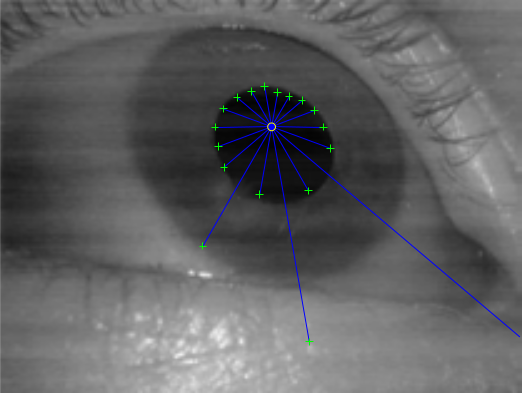
\includegraphics[width=.31\textwidth]{./Pictures/3a.png}
        }
        \subfigure[Stage 2 inlier point]{
           \label{fig:stage_2_inlier}
           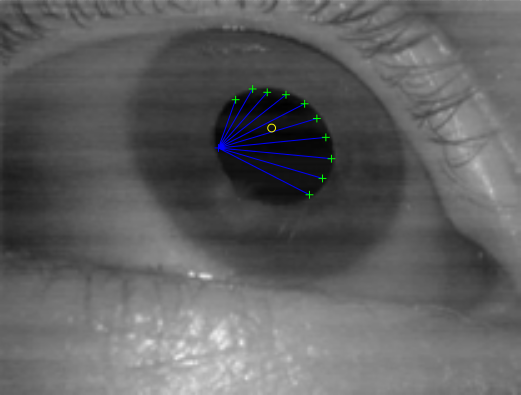
\includegraphics[width=.31\textwidth]{./Pictures/3b.png}
        }
        \subfigure[Stage 2 outlier point]{
            \label{fig:stage_2_outlier}
            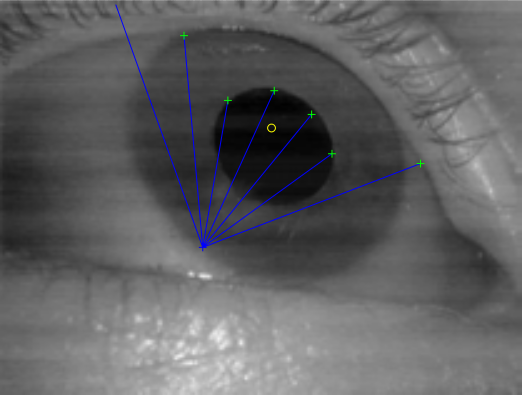
\includegraphics[width=.31\textwidth]{./Pictures/3c.png}
       }
   }
   \caption{Visualization of Starburst stage 1 and stage 2 feature point detection procedure \label{fig:starburst_example} }   
\end{dBox}   
\end{figure*}

For every feature point obtained the above described algorithm is repeated with a minor modification. Search rays are limited to $\gamma = \pm 50$ degrees from the original ray that originally produced the feature point. This procedure tends to increase the ratio of the number of feature points on the pupil contour over the number of feature points not on the pupil contour. If the pivot feature point lies on the pupil contour then the rays around the original ray will result in feature points that also lie on the opposite half of the pupil contour. On the other hand if the original feature point is not on the pupil contour, then limiting the search space will cut down the number of feature point that doesn't lie on the pupil contour. One important note to take into consideration is that the number of rays in this step is only 10 (5 on each side of the original ray). Figure \ref{fig:starburst_stage2_example} shows the two cases described above. \bigskip



\begin{figure*}[h]
\begin{dBox}
\centering
  \mbox{
        \subfigure[Stage 2 inlier point]{
           \label{fig:stage_2_inlier_p}
           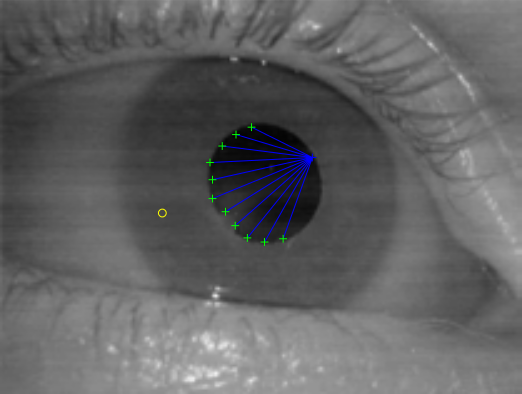
\includegraphics[width=.31\textwidth]{./Pictures/4b.png}
        }
        \subfigure[Stage 2 outlier point]{
            \label{fig:stage_2_outlier_p}
            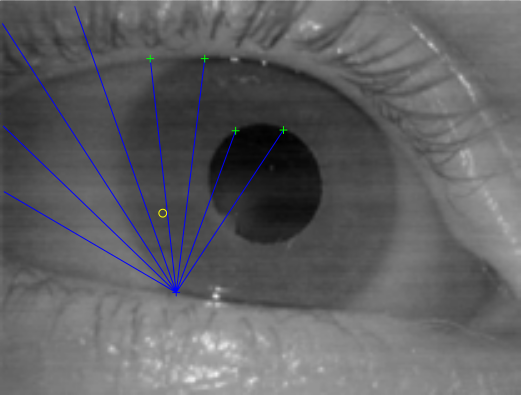
\includegraphics[width=.31\textwidth]{./Pictures/4c.png}
       }
   }
   \caption{Visualization of Starburst stage 2 feature point detection procedure \label{fig:starburst_stage2_example} }   
\end{dBox}   
\end{figure*}

Using the two stage feature detection process improves the robustness of the method to poor initial guesses for the starting point. However, the feature points tend to bias to the side of the pupil contour nearest the initialization point. Although another iteration of the ray process would minimize this bias, the computational burden grows exponentially with each iteration and thus would be an inefficient strategy. \bigskip

Fitting an ellipse to the set of biased feature points will induce significant error into fit. A good strategy to eliminate the bias is to iterate the recently described procedure, with each time computing the average of the detected feature points to be the new estimated center of the pupil for the next iteration. The iterating process is halted when the estimated pupil center between two successive iteration is less than $d = 10$ pixels. Starburst paper mention that if guess is a good estimate of the pupil center, only a single iteration is required. When the initial estimate is not good, typically only a few iterations ($< 5$) are required for convergence. If convergence is not reached within $i = 10 $iterations, as occurs sometimes during a blink when no pupil is visible, the algorithm halts and begins processing the next frame. \bigskip

In out implementation of this module we sticked to the exact Startburst algorithm described in the paper.



\section{Ellipse Fitting}{Ellipse Fitting}
Given a set of feature points, the function of this module is to find best fitting ellipse.  Most of algorithms use least-squares ellipse fitting including all feature points (e.g. see \cite{least_squares}). Using all points to estimate an ellipse results in significant error that strongly affect the accuracy. Notice that a few feature points not on the pupil contour dramatically reduces the quality of the fit to an unacceptable level.  \bigskip

To address this issue Starburst uses Random Sample Consensus (RANSAC) paradigm for model fitting \cite{ransac}. Starburst paper claims that Starburst is the first algorithm that uses RANSAC in the context of eye-tracking. RANSAC is an effective technique for model fitting in the presence of a large but unknown percentage of outliers in a measurement sample. A basic assumption is that the data  consists of "inliers", i.e., data whose distribution can be explained by some set of model parameters, though may be subject to noise, and "outliers" which are data that do not fit the model. In our application inliers are feature points that lie on the pupil contour, while outliers are feature points that belong to other contours other than the pupil contour. Least-squares approaches assumes that all sample points fit the model and hence, uses all the sample points to estimate the model. On the other hand RANSAC is an iterative method to estimate parameters of a mathematical model from a set of observed data which contains outliers. General outline of RANSAC technique is shown at algorithm \ref{ransac_outline}. \bigskip

\begin{algorithm}
\begin{dBox}
	\caption{General RANSAC Procedure} \label{ransac_outline}
	\begin{algorithmic}[1]
		\Procedure{RANSAC}{}
		 \While{$i < N$}
			\State Draw $s$ points uniformly at random
			\State Fit model to these $s$ points
			\State Find inliers to this model among the remaining points (points whose error $ < t$)
			\State If there are $d$ or more inliers, accept the model and refit using all inliers	
		\EndWhile	
		\EndProcedure	
	\end{algorithmic}
\end{dBox}	
\end{algorithm}


The output of the two stage feature detection process may result in very few outliers in some cases, while in other cases outlier prevail. Using the RANSAC technique increase the ability of the system to do robust estimation of the model (ellipse) parameters. The following procedure is repeated $R$ times. First, five samples are randomly drawn from the set of feature set obtained by the previous module.  Singular Value Decomposition (SVD) on the conic constraint matrix generated with normalized feature-point coordinates \cite{multipleViewGeom} is used to find the parameters of the ellipse that perfectly fit these five points. Then, the number of candidate feature points in the data set that agree with this model (i.e. the inliers) are counted. Inliers are those sample points for which the algebraic distance to the ellipse is less than some threshold $t$. \bigskip

Our implementation of this stage differs a bit from the implementation of the original Starburst. We draw 5 samples from the detected feature set, then we compute the best fit ellipse using Fitzgibbon's algorithm \cite{fitzgibbon96} which is implemented in OpenCV. Finally we evaluate the error between the estimated model and all feature points and count inliers/outliers. Algorithm \ref{our_ransac_outline} summarizes how we use RANSAC in our system. \bigskip

\begin{algorithm}
\begin{dBox}
	\caption{Our RANSAC Procedure} \label{our_ransac_outline}
	\begin{algorithmic}[1]
		\Procedure{RANSAC}{}
		 \While{$i < N$}
			\State Draw $s$ points uniformly at random
			\State Fit ellipse model to these $s$ points
			\State Find inliers to this ellipse (points whose algebraic error $ < t$)
			\State If there are $d$ or more inliers, accept the ellipse and refit using all inliers	
		\EndWhile	
		\EndProcedure	
	\end{algorithmic}
\end{dBox}	
\end{algorithm}


As a matter of fact we tried different approaches in our implementation, at first we tried to implement the same approach mentioned in the Starburst paper. However finding the SVD of the parameter matrix using OpenCV SVD didn't produce consistent results because the calculated eigen vectors/values were not correct. Some books like \cite{practicalOpenCV} addressed this issue and suggested using Eigen mathematics library \cite{eigenweb} to find the eigen values/vector. In our application we couldn't benefit from this solution since, Eigen library is only available in C++ while the user end if our application is in Java (Android user end).


\subsection{Estimation of Number of Iterations $R$}\index{Number of Iterations}
Starbusrt algorithm assumes that the average error variance of the feature detector is approximately one pixel and that this error is distributed as a Gaussian with zero mean. Thus to obtain a 95\% probability that a sample is correctly classified as an inlier, the threshold should be derived from a $\chi^{2}$ distribution with one degree of freedom \cite{multipleViewGeom}. This results in a threshold distance of $t = 1.98$ pixels. \bigskip

The parameter R (the number of iterations), however, can be determined from a theoretical result. Let p be the probability that the RANSAC algorithm in some iteration selects only inliers from the input data set when it chooses the $s$ points from which the model parameters are estimated. When this happens, the resulting model is likely to be useful so $p$ gives the probability that the algorithm produces a useful result. Let $w$ be the probability of choosing an inlier each time a single point is selected, that is, 
\begin{dBox}
	$$ w = \frac{number \: of \: inliers \: in \: data}{number \: of \: points \: in \: data} $$
\end{dBox}
it can be proven that 
\begin{dBox}
\begin{equation}
		R = \frac{log(1-p)}{log(1-w^{5})}
\end{equation}
\end{dBox}

\section{Homographic Mapping and Calibration}\index{Homographic Mapping and Calibration}
In order to calculate the point of gaze of the user in the scene image, a mapping between locations in the scene image and an eye-position measure must be determined. The typical way to determine the mapping is via a calibration process. During calibration, the user is required to look at a number of scene points for which the positions in the scene image are known. At each position the eye-position $\vec{e} = (x_{e} ,\: y_{e},\: 1)$ and the scene position $\vec{s} = (x_{s},\: y_{s},\: 1)$ is measured. The mapping is generated using the $3x3$ Homography matrix which has 8 degrees of freedoms. Each point (map from scene to eye) produces 2 independent equations. Hence four mapping points are needed to compute the entries of the homography matrix up to scale \cite{heuristic}. \bigskip

In our implementation we use the OpenCV \textit{findHomography} procedure to find the homography matrix. Given a set of points in image coordinates and corresponding set of points in the eye coordinates, \textit{findHomography} finds a perspective transformation between two coordinate systems. \bigskip

Once this mapping is determined the user’s point of gaze in the scene for any frame can be established
as $\vec{s} = H \vec{e}$.


\chapterimage{eyes_women_cropped.jpg}
\chapter{MIRT Morphological Based Iris Tracking Algorithm}
In this chapter we present a novel method for real-time iris detection and tracking MIRT. MIRT is morphological based real-time iris detection algorithm. Morphological operations are simple and fast to compute which reduces the time required to detect the iris.

\section{Overview}\index{Overview}
MIRT algorithm is composed of 2 stages; 1) location region of interest in the given image, and 2) detecting the iris in the region of interest located in stage 1. 



%----------------------------------------------------------------------------------------
%	CHAPTER 3 // Pupil Eye Tracking Algrithm
%----------------------------------------------------------------------------------------
\chapterimage{Pupil_Chapter_photo4.jpg}
\chapter{Pupil Eye Tracking Algorithm}
As proposed in the previous chapters that we rely on Starburst Algorithm to get the center of the pupil. But we found that Starburst is not robust and accurate, so we will use Pupil Algorithm to enhance eye-tracking module. Through this chapter we will go through the details of our eye-tracking module by using Pupil Algorithm.

\section{Pupil}\index{Pupil}
In the second version of our eye-tracking module we went for implementing the Pupil Algorithm \cite{pupil}. Pupil eye-tracking algorithm is an accessible, affordable and extensible tool for pervasive eye tracking research. This chapter we will explain the design motivation of the algorithm, provide an in depth technical description of software. We will use a wearable mobile eye tracking headset with one 
scene camera and one infra-red (IR) spectrum eye camera for dark pupil detection. Both cameras connect to a laptop, desktop, or mobile computer platform via high speed USB 2.0. The camera video streams are read for real-time pupil detection, gaze mapping and recording.  


\section{System Design Objectives}\index{Pupil}
	Pupil leverages the rapid development cycle and scaling effects of consumer electronics, USB cameras and consumer computing hardware, instead of using custom cameras and computing solutions. \bigskip

Pupil algorithm is open source and strives to build and support a community of eye tracking researchers and developers.

\section{Cameras} \index{Cameras}
The scene camera mount and eye camera mount interface geometries are open source. By releasing the mount geometry we automatically document the interface, allowing users to develop their own mounts for cameras of their choice. \bigskip

Pupil uses USB interface digital cameras that comply with the UVC (USB Video Class) standard. The Pupil headset can be used with other software that supports the UVC interface. Pupil can be easily extended to use two eye cameras for binocular set-ups and more scene cameras as desired. 

\subsection{Eye Camera} \index{Eye Camera}
We use a small and lightweight eye camera to reduce the amount of visual obstruction for the user and keep the headset lightweight. The eye camera can capture at a maximum resolution of 800x600 pixels at 30 Hz. Using an IR mirror ("hot mirror") was considered as  strategy to further reduce visual obstruction. 

\bigskip
 Pupil uses the "dark pupil" detection method. This Requires the eye camera to capture video within a specific range of the IR spectrum. 
 
 \subsection{Scene Camera} \index{Eye Camera}
  The scene camera is mounted above the user’s eye aligning the scene camera optics with the user’s eye along a sagittal plane. The scene camera faces outwards to capture a video stream of a portion of the users FOV at 30Hz. The scene camera lens has a 90 degree diagonal FOV. The scene camera is not only high resolution (max resolution 1920x1080 pixels), but also uses a high quality image sensor. This is very
advantageous for further computer vision and related tasks
performed in software.


\section{Computing Device} \index{Computing Device}
The Pupil eye tracking algorithm works in conjunction with standard multi-purpose computers: laptop, desktop, or tablet. Designing for user supplied recording and processing hardware introduces a source for compatibility issues and requires more set-up effort for both users and developers. However, enabling the user to pair the headset with their own computing platform makes Pupil a multi-purpose eye tracking and analysis tool. Pupil is deployable for lightweight mobile use as well as more specialized applications like: streaming over networks, geotagging, multi-user synchronization; and computationally intensive applications like real time 3D reconstruction and localization.

\section{Pupil Detection Algorithm} \index{Pupil Detection Algorithm}
The pupil detection algorithm locates the dark pupil in the IR illuminated eye camera image. The algorithm does not depend on the corneal reflection, and works with users who wear contact lenses and eyeglasses. \bigskip

The pupil detection algorithm is under constant improvement based on feedback collected through user submitted eye camera videos. Here we provide a description of default pupil detection algorithm.
\bigskip

\subsection{overview} \index{Pupil Detection Algorithm}
The eye camera image is converted to gray-scale. The initial region estimation of the pupil is found via the strongest response for a center-surround feature as proposed by Swirski et al. \cite{Swirski} within the image. \newline  

Detect edges using Canny \cite{Canny} to find contours in eye image. Filter edges based on neighbouring pixel intensity. Look for darker areas (blue region). Dark is specified using a user set offset of the lowest spike in the histogram of pixel intensities in the eye image. \\*

Filter remaining edges to exclude those stemming from spectral reflections. Remaining edges are extracted into into contours using connected components \cite{Suzuki}. Contours are filtered and split into sub-contours based on criteria of curvature continuity. \\*

Candidate pupil ellipses are formed using ellipse fitting \cite{Fitzgibbon} onto a subset of the contours looking for good fits in a least square sense, major radii within a user defined range, and a few additional criteria. \\* 

The results are evaluated based on the ellipse fit of the supporting edges and the ratio of supporting edge length and ellipse circumference (using Ramanujans second approximation \cite{Ramanujans} ). We call this ratio "confidence". If the best results confidence is above a threshold the algorithm reports this candidate ellipse as the ellipse defining the contour of the pupil. Otherwise the algorithm reports that no pupil was found.\\*

\begin{figure*}[]
\begin{dBox}
\centering
  \mbox{
	    \subfigure[Algorithm Overview]{
            \label{fig:overview}
            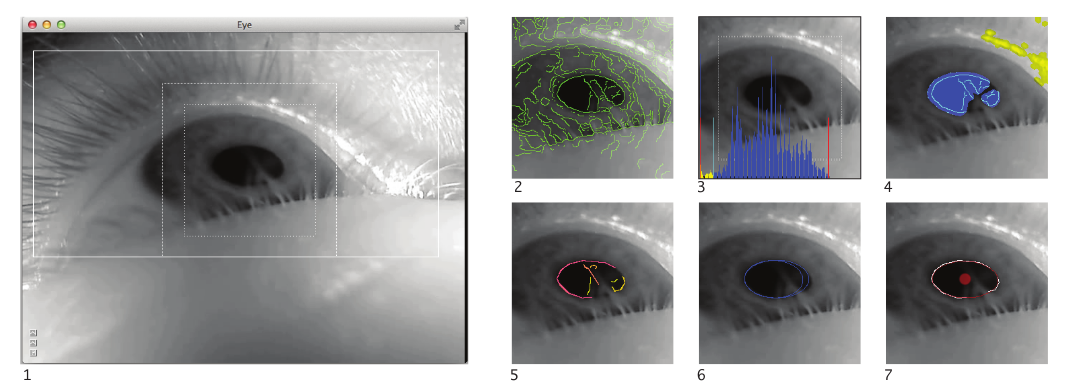
\includegraphics[width=1.0\textwidth]{./Pictures/Visulaization_of_Pupil_algo.png}
        }
   }
   \caption{Vizualization of pupil detection algorithm. 1) Eye image converted to gray scale, user region of interest (white stroke rectangle), and initial estimation of pupil region (white square and dashed line square.) 2) Canny edge detection (green lines). 3) Define "dark" region as offset from lowest spike in histogram within eye image. 4) Filter edges to exclude spectral reflections(yellow) and not inside "dark" areas (blue). 5) Remaining edges extracted into contours using connected components and split into sub-contours based on curvature criteria (multi colored lines). 6) Candidate pupil ellipses (blue) are formed using ellipse fitting. 7) Final Ellipse fit found through an augmented combinatorial search( finally ellipse with center in red)-supporting edge pixels drawn in white.
 \label{fig:Pupil_Performance} }   
\end{dBox}   
\end{figure*}


\begin{figure*}[]
\begin{dBox}
\centering
  \mbox{
	      \subfigure[Comparison]{
            \label{fig:Comparison}
            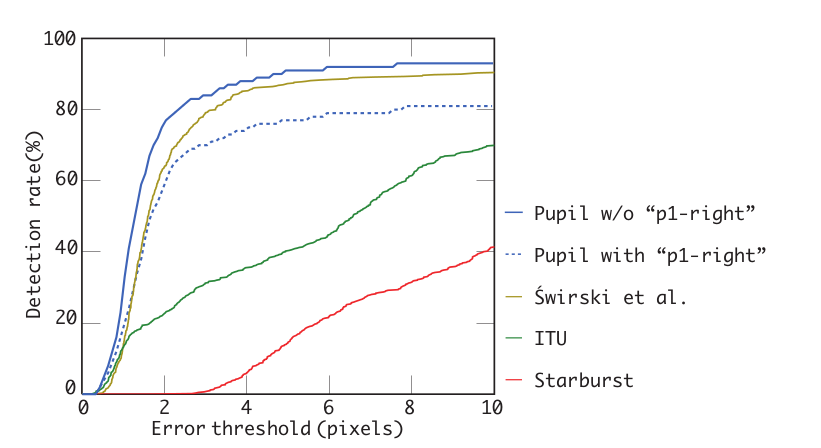
\includegraphics[width=.80\textwidth]{./Pictures/comparison.png}
        }
   }
   \caption{Comparison of pupil detection rate for Pupil’s algorithm, the stock algorithm proposed by 					Swirski et al., the ITU gaze tracker and Starburst.
 \label{fig:Pupil_Performance} }   
\end{dBox}   
\end{figure*}

Figure \ref{fig:Pupil_Performance} shows a performance comparison between Pupil’s pupil detection algorithm, the stock algorithm proposed by Swirski et al., the ITU gaze tracker and Starburst on the benchmark dataset by Swirski et al. \cite{DataSet}. As error measure we used the Hausdorff distance between the detected and hand-labeled pupil ellipses. We additionally conducted a test excluding the dataset p1-right, that contains eye images recorded at the most extreme angles.
As can be seen from the Figure, Pupil without p1-right compares favourably to all other approaches. With an error threshold of 2 pixels Pupil achieves a detection rate of 80\%; at 5 pixels error detection rate increases to 90\%

\begin{figure*}[]
\begin{dBox}
\centering
  \mbox{
	      \subfigure[Initial Estimation of Pupil Region]{
            \label{fig:Pupil Region}
            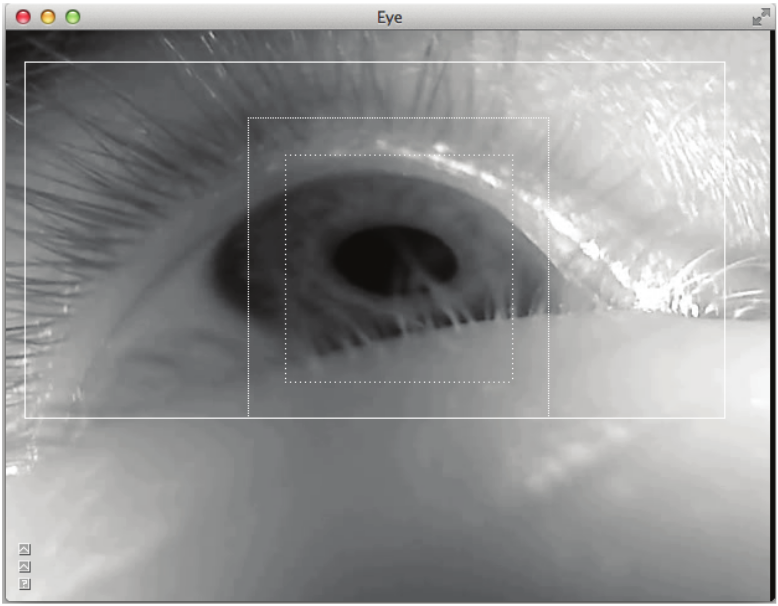
\includegraphics[width=.80\textwidth]{./Pictures/initial_estimation_of_pupil.png}
        }
   }
   \caption{ User region of interest (white stroke rectangle), and initial estimation of pupil region (white square and dashed line square.)
 \label{fig:Pupil Region} }   
\end{dBox}   
\end{figure*}


\begin{figure*}[]
\begin{dBox}
\centering
  \mbox{
	      \subfigure[Estimation of Pupil Region]{
            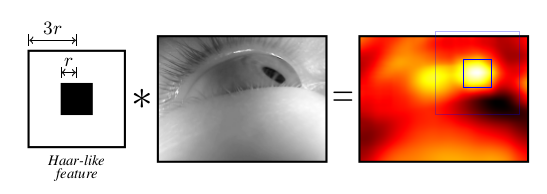
\includegraphics[width=.80\textwidth]{./Pictures/estimation_pupil_region.png}
        }
   }
   \caption{ To find the approximate pupil region, the eye image is convolved with a Haar-like centre surround feature of radius r. The pupil region is centred on the location of the maximal response over all pixels and radii
 \label{fig:EstimationPupilFig} }   
\end{dBox}   
\end{figure*}


\begin{figure*}[]
\begin{dBox}
\centering
  \mbox{
	      \subfigure[]{
            \label{fig:IntegralImage}
            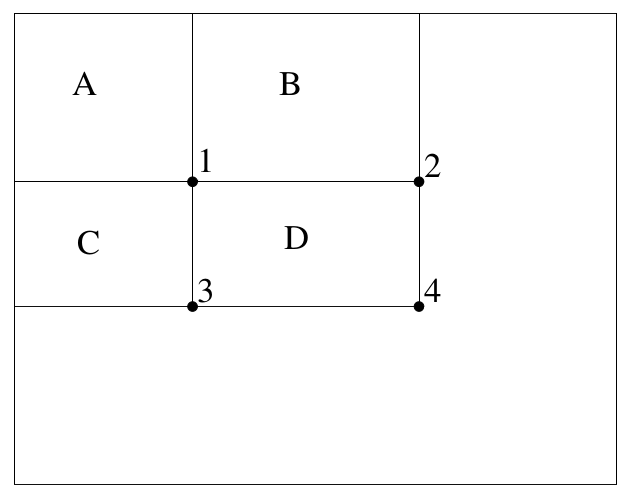
\includegraphics[width=.40\textwidth]{./Pictures/integral_image.png}
        }
   }
   \caption{ To find the approximate pupil region, the eye image is convolved with a Haar-like centre surround feature of radius r. The pupil region is centred on the location of the maximal response over all pixels and radii
 \label{fig:IntegralFig} }   
\end{dBox}   
\end{figure*}


\subsection{Integral Image} \index{ Pupil Detection Algorithm }
Rectangle features can be computed very rapidly using an intermediate representation for the image which we call the integral image. The integral image at location $x, y$ contains the sum of the pixels above and to the left of $x, y$, inclusive: \\
\begin{center}
$ii(x,y)=\sum\limits_{x'<=x,y'<= y}i(x', y')$,
\end{center}
where $ii(x,y)$ is the integral image and $i(x,y)$ is the original image. Using the following pair of recurrences:
\begin{center}
	\begin{equation}
	$s(x,y) = s(x,y-1)+ i(x,y)$
	\end{equation}

	\begin{equation}
	$ii(x,y) = ii(x-1,y)+ s(x,y)$
	\end{equation}

\end{center}
(where $ s(x,y) $is the cumulative row sum, $s(x, -1) = 0$, and $ii(-1, y) == 0$) the integral image can be computed in one pass over the original image. \\
Using the integral image any rectangular sum can be computed in four array references figure \ref{fig:IntegralFig}. Clearly the difference between two rectangular sums can be computed in eight references. Since the two-rectangle features defined above involve adjacent rectangular sums they can be computed in six array references, eight in the case of the three-rectangle features, and nine for four-rectangle features.

\begin{figure*}[]
\begin{dBox}
\centering
  \mbox{
	      \subfigure[Original Eye Image]{
	            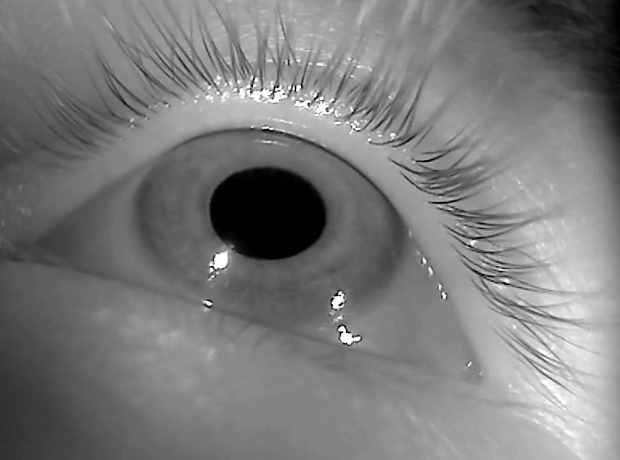
\includegraphics[width=.45\textwidth]{./Pictures/0-eye.png}
        }
	      \subfigure[Region of interest(ROI) after Running Initial Estimation Of Pupil Module]{
	      		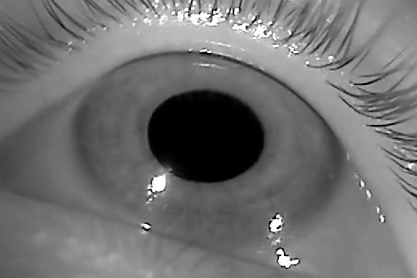
\includegraphics[width=.50\textwidth]{./Pictures/ROI.png}
        }
   }
   
   \caption{Input \& Output of Initial Estimation of Pupil Module. \label{fig:Initial_Estimation_Of_Pupil} }   
\end{dBox}   
\end{figure*}

\subsection{Initial Estimation Of Pupil} \index{Pupil Detection Algorithm}
Our initial region estimation assumes that the pupil region, either the dark pupil itself or the combination of pupil and iris, can roughly be described as a “ dark blob surrounded by a light background ”, and is the strongest such feature in the image. To find the pupil, we use a Haar-like feature detector, similar to the features used in cascade classifiers [Viola and Jones 2001]. \bigskip

The core idea of the feature detector can be explained in terms of convolution. To find possible pupil regions, we convolve the image with a Haar-like centre-surround feature of a given radius figure \ref{fig:EstimationPupilFig} . We repeat this for a set of possible radii, between a user specified minimum and maximum, and find the strongest response over the 3D space of (x, y) and radii. The (x, y) location of this strongest response is assumed to be the centre of the pupil region, with the size of the region determined by the corresponding radius. \bigskip

Although such a convolution is a slow operation if performed naively, we optimise this by first calculating the integral image [Viola and Jones 2001]. Using this integral image, we can find the response of a pixel to a Haar-like feature in constant time, only needing to sample 8 pixel values, one for each corner of the two squares, thereby making this step linear in the number of pixels and possible radii. \\
Input and Output of this module is shown in Figure \ref{fig:Initial_Estimation_Of_Pupil}

\begin{figure*}[]
\begin{dBox}
\centering
  \mbox{
	      \subfigure[Eye Image after Computing Histogram]{
	            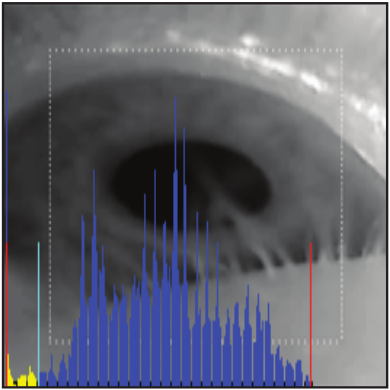
\includegraphics[width=.40\textwidth]{./Pictures/histogramOnDarkRegion.png}
        }
   }
   \caption{After Computing Histogram to get Spikes. 
   \label{fig:HistogramOnEyeImage} }   
\end{dBox}   
\end{figure*}

\begin{figure*}[]
\begin{dBox}
\centering
  \mbox{
	    \subfigure[Eye image after applying Closing operation on Eye image.]{
	          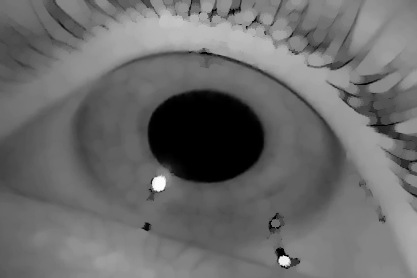
\includegraphics[width=.60\textwidth]{./Pictures/dark_region_img.png}
        }
        	\subfigure[Dark region is indicated by the Blue Region]{
        		  \label{fig:SpectralReflection} 
	          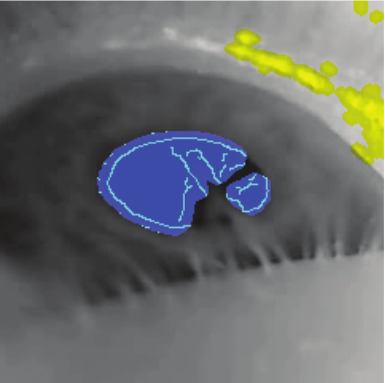
\includegraphics[width=.40\textwidth]{./Pictures/DarkRegion.png}
        }

   }
   \caption{After Applying Morphological operations(Closing operations). 
   \label{fig:DarkImageInBlue} }   
\end{dBox}   
\end{figure*}


\begin{figure*}[]
\begin{dBox}
\centering
  \mbox{
	    \subfigure[Eye image after applying Closing operation on Eye image.]{
	          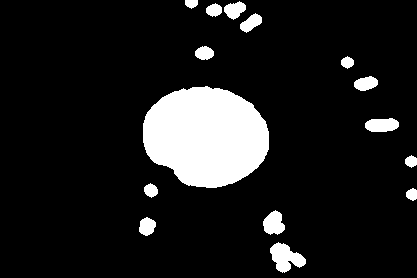
\includegraphics[width=.30\textwidth]{./Pictures/dark_region_binary_img.png}
        }
   }
   \caption{Final Result of Getting Dark Region Module. 
   \label{fig:DarkImageInBinary} }   
\end{dBox}   
\end{figure*}


\subsection{Getting Dark Region(Pupil Region)} \index{Pupil Detection Algorithm}
Here we want to extract the region which include the pupil by getting the most dark region in eye image. And then we filter the eye image by applying some Morphological operations like Dilation and Erosion to remove the noise to get a pure dark region. \bigskip

At first we should get the histogram of the gray image of Region Of Interest (ROI) which we get from Initial Estimation Of Pupil Module. Then we should deduce spikes from histograms. After getting the lowest and highest spikes in histogram we can get the binary image of ROI by using lowest spike +  user offset(usually we set offset by 11) as threshold as shown in figure \ref{fig:HistogramOnEyeImage}. \bigskip

Then, we should do some Morphological operation on binary image. to filter the image from any noise and make contours more clearer, so we apply Erosion at first and then Dilation(Closing Operation) as shown in Figure \ref{fig:DarkImageInBlue}. \bigskip

Finally we get the ROI as a binary image include only the Dark Region which represents Pupil as shown in Figure \ref{fig:DarkImageInBinary}.


\begin{figure*}[]
\begin{dBox}
\centering
  \mbox{
	    \subfigure[Edges of eye image after Excluding Spectral Reflections]{
	          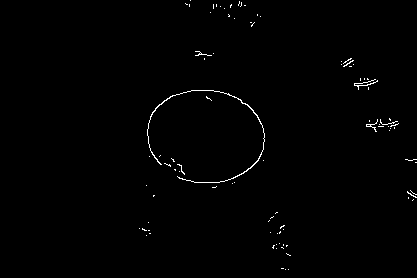
\includegraphics[width=.50\textwidth]{./Pictures/edges_after_Removing_Spectral_Refl.png}
        }
   }
   \caption{Final Result of Excluding Spectral Reflection module.
   \label{fig:Edges} }   
\end{dBox}   
\end{figure*}

\subsection{Excluding Spectral Reflection} \index{Pupil Detection Algorithm}
	We need to filter all the edges which result from Canny edge detector, by excluding the spectral reflection which appears as yellow lines in figure \ref{fig:SpectralReflection} that is out of the dark region. So, we need to remove edges in areas which are not dark enough and where the glints is (Spectral Reflection from IR leds).\bigskip
		
	We get minimum edges from comparing edges image which result from Canny edge detector with the Spec Mask (Mask that we get from the in range thresholding with highest spike and 255) and then we reduce the number of edges by comparing the edges image with binary Mask(Mask which we get from in range thresholding with lowest spike with 255).\bigskip

	At the end we remove the Spectral reflection and the binary eye image is filtered from any noise as shown in Figure \ref{fig:Edges}. 
	 


\begin{figure*}[]
\begin{dBox}
\centering
  \mbox{
	    \subfigure[Multi coloured lines represent different contours ]{
	          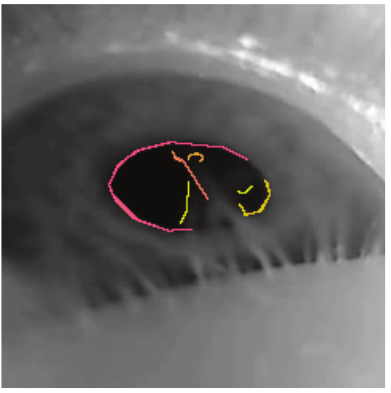
\includegraphics[width=.30\textwidth]{./Pictures/contours.png}
        }
   }
   \caption{Final Result of Extracting Contour module.
   \label{fig:Contours} }   
\end{dBox}   
\end{figure*}


\subsection{Extracting Contours} \index{Pupil Detection Algorithm}
	After getting the minimum edges we can extract Contours by using connected components, and then split the contours into sub-contours based on curvature continuity criteria as shown in Figure \ref{fig:Contours}. \bigskip
	We have used OpenCV findCountours method to get all the contours from edges and then we get the approximate Poly-lines that each contour forms. So that, we can use each poly-line to get the angle between each subsequent 2 points to make sure that this contour is a good contour and also it helps to split contours into sub-contours based on angles between two subsequent points.  


\begin{figure*}[]
\begin{dBox}
\centering
  \mbox{
	    \subfigure[Final ellipse with center in red and supporting edge pixels are drawn in white.]{
	          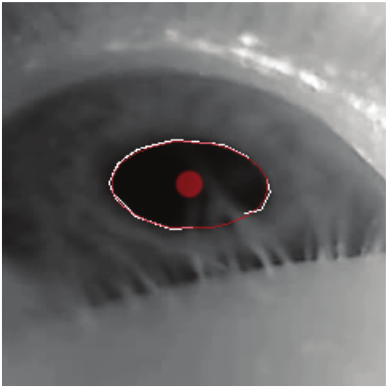
\includegraphics[width=.30\textwidth]{./Pictures/final_ellipse.png}
        }
   }
   \caption{Final Result of Ellipse Fitting module.
   \label{fig:EllipseFit} }   
\end{dBox}   
\end{figure*}


\subsection{Ellipse Fitting} \index{Pupil Detection Algorithm}
	Finally we should estimate the best ellipse that surrounds the Pupil by fitting an ellipse found through an augmented combinatorial search. \bigskip
	
	Candidate pupil ellipses are formed using ellipse fitting onto a subset of the contours looking for good fits in a least square sense, major radii within a user defined range and a few additional criteria. An augmented combinatorial search looks for contours that can be added as support to the candidate ellipses. The results are evaluated based on the ellipse fit of the supporting edges and the ratio of supporting edge length and ellipse circumference. We call this ratio “ confidence ”. If the best results confidence is above a threshold the algorithm reports this candidate ellipse as the ellipse defining the contour of the pupil as shown in Figure \ref{fig:EllipseFit}. Otherwise the algorithm reports that no pupil was found. \bigskip
	
	
 
	 














%----------------------------------------------------------------------------------------
%	BIBLIOGRAPHY
%----------------------------------------------------------------------------------------

% \chapter*{Bibliography}
% \addcontentsline{toc}{chapter}{\textcolor{ocre}{Bibliography}}
\printbibliography[]



% \section*{Books}
% \addcontentsline{toc}{section}{Books}
% \printbibliography[heading=bibempty,type=book]
% \section*{Articles}
% \addcontentsline{toc}{section}{Articles}
% \printbibliography[heading=bibempty,type=article]

%----------------------------------------------------------------------------------------
%	INDEX
%----------------------------------------------------------------------------------------

\cleardoublepage
\phantomsection
\setlength{\columnsep}{0.75cm}
\addcontentsline{toc}{chapter}{\textcolor{ocre}{Index}}
\printindex

%----------------------------------------------------------------------------------------

\end{document}